% !TeX root = it-governance-risk-compliance.tex
% !TeX encoding = UTF-8
\chapter{COBIT 2019: Sistem Tata Kelola dan Faktor Desain}

\section*{Tujuan Pembelajaran}
\begin{itemize}
  \item Menjelaskan komponen sistem tata kelola dan 40 objektif tata kelola dan
  manajemen dalam COBIT 2019.
  \item Menerapkan faktor desain dan \textit{goals cascade} untuk memilih objektif yang
  paling penting bagi sebuah organisasi.
  \item Menilai tingkat kapabilitas saat ini untuk objektif prioritas berdasarkan bukti,
  bukan pengakuan.
\end{itemize}

\section{Pendahuluan}

Misalkan rapat komite pengarah teknologi informasi (TI) Medikara membahas temuan audit
internal: 6 dari 30 akun vendor yang diperiksa masih aktif setelah penugasan berakhir.
Direktur utama menutup rapat dengan satu kalimat: ``Terapkan COBIT.'' Kepala TI membuka
daftar 40 objektif dan tidak tahu harus mulai dari mana. Konsultan menawarkan penilaian
seluruh objektif dengan hasil satu angka rata-rata. Direktur pelayanan bertanya apakah angka
itu akan memperpendek antrean, dan tidak ada yang bisa menjawab. Organisasi sering
menyatakan akan menerapkan COBIT tanpa menjelaskan masalah yang hendak diselesaikan.
Hasilnya dapat berupa puluhan prosedur baru sementara akses vendor tetap tidak ditinjau.
Kesulitan itu muncul karena kerangka diperlakukan sebagai daftar pekerjaan seragam bagi
semua organisasi.

COBIT adalah Control Objectives for Information and Related Technologies. Bab ini
menggunakan model inti COBIT 2019 sebagai bahasa untuk memilih objektif, menilai
kapabilitas, dan merancang perbaikan. Tujuan awal bukan memperoleh nilai rata-rata
tinggi, melainkan mengetahui proses mana yang paling memengaruhi layanan dan bukti apa
yang mendukung penilaian. Bab ini juga membuka tonggak C2 Kondisi Saat Ini. Tim capstone
menghasilkan lembar faktor desain, rantai tujuan, lima sampai tujuh objektif prioritas, dan
potret kapabilitas.

Rujukan utama adalah buku pengantar dan panduan desain COBIT 2019 dari ISACA. Akses ke
terbitan resmi itu terbatas, sehingga rincian yang dapat diperiksa mahasiswa diambil dari
artikel terbuka di situs ISACA dan dua studi rumah sakit di Indonesia. Bagian yang merupakan
tafsir penulis ditandai dengan frasa ``penafsiran bab ini''. Pembacaan harus membedakan
model COBIT 2019 dari COBIT 5 dan dari COBIT 7 yang diumumkan pada Oktober 2026
\cite{cobit2019-intro,cobit2019-design,c04-perbandingan,c04-denpasar,c04-wilujeng,c04-transisi}.

\IfFileExists{../figures/ch04-diagram-konsep.png}{%

Gambar \ref{fig:ch04-ilustrasi-bab} merangkum hubungan komponen dan konsep utama bab ini.
\begin{figure}[!htb]
  \centering
  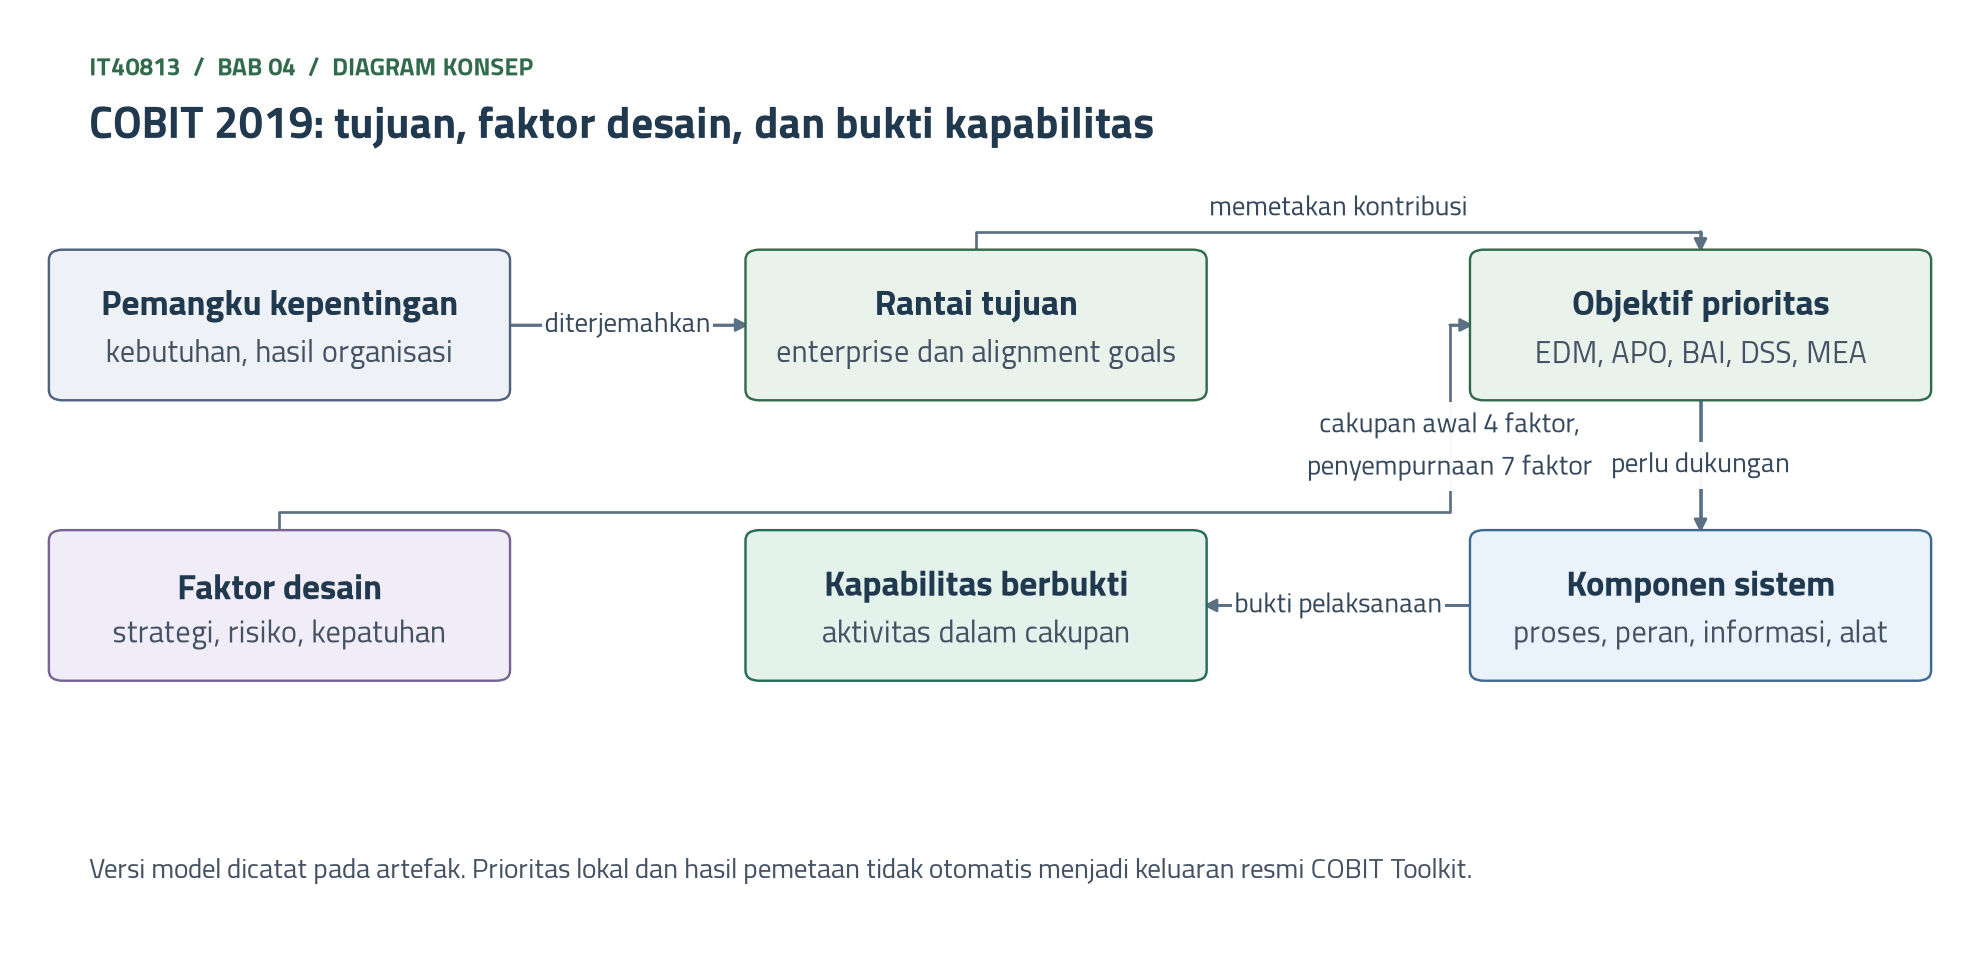
\includegraphics[width=\textwidth]{../figures/ch04-diagram-konsep.png}
  \caption{COBIT 2019: tujuan, faktor desain, dan bukti kapabilitas}
  \label{fig:ch04-ilustrasi-bab}
\end{figure}
}{}

\section{COBIT 2019 sebagai Kerangka Tata Kelola}

COBIT 2019 adalah kerangka tata kelola dan manajemen informasi serta teknologi dari ISACA.
Kerangka ini memuat prinsip, komponen, model inti berisi 40 objektif pada lima domain, serta
panduan merancang sistem tata kelola \cite{c04-baru,c04-halaman}. Cara kerjanya: organisasi
memakai konteksnya untuk memilih bagian model yang paling penting, lalu menilai pelaksanaan
bagian itu. Isi COBIT bersifat umum dan perlu disesuaikan \cite{c04-sistematis}.
Tabel~\ref{tab:ch04-publikasi} memperlihatkan empat publikasi inti dan pertanyaan yang
dijawab masing-masing \cite{cobit2019-intro,c04-gmo,cobit2019-design,c04-implementasi}. Dua
publikasi desain dan implementasi sudah menyatakan arahnya pada judul: merancang serta
menerapkan solusi, bukan menyalin isi model.

\begin{table}[!htb]
  \centering\small
  \caption{Empat publikasi inti COBIT 2019}\label{tab:ch04-publikasi}
  \begin{tabularx}{\textwidth}{|>{\raggedright\arraybackslash}p{0.36\textwidth}|>{\raggedright\arraybackslash}X|>{\raggedright\arraybackslash}p{0.17\textwidth}|}
    \hline
    \textbf{Publikasi} & \textbf{Pertanyaan yang dijawab} & \textbf{Seksi bab ini} \\ \hline
    Framework: Introduction and Methodology & Apa konsep dan prinsip kerangka ini? & Prinsip,
    komponen \\ \hline
    Framework: Governance and Management Objectives & Apa isi tiap objektif, praktik, dan
    aktivitasnya? & Model inti, kapabilitas \\ \hline
    Design Guide & Bagaimana merancang sistem sesuai konteks organisasi? & Faktor desain, rantai
    tujuan \\ \hline
    Implementation Guide & Bagaimana menerapkan dan mengoptimalkan rancangan itu? & Dibahas lagi
    pada C4 \\ \hline
  \end{tabularx}
\end{table}

Cara berpikirnya mirip bengkel mobil. Katalog bengkel memuat ratusan suku cadang. Pemilik mobil
tidak mengganti semuanya. Montir mendengar keluhan, memeriksa mobil, lalu memilih bagian yang
perlu diperbaiki. Katalog membantu menyebut nama bagian, tetapi katalog bukan rencana perbaikan.

Dua contoh kasus nyata:
\begin{enumerate}
  \item Kadam menelusuri satu tujuan organisasi tentang kelangsungan layanan. Empat objektif
  yang dipilih memuat 25 praktik dan 140 aktivitas \cite{c04-kontinuitas}. Rata-ratanya 35
  aktivitas per objektif. Misalkan rata-rata itu berlaku untuk seluruh model, sehingga 40
  objektif memuat sekitar 1.400 aktivitas. Ini perkiraan kasar, bukan hitungan resmi. Bila satu
  aktivitas diperiksa 30 menit, penilaian menyeluruh menghabiskan 700 jam atau 87,5 hari kerja
  satu orang. Empat objektif hanya memerlukan 70 jam atau 8,75 hari kerja.
  \item Bab 1 sudah menghitung bahwa 52 staf TI Medikara yang dibagi ke 40 objektif hanya
  menghasilkan 1,3 orang per objektif. Bila dibagi ke 6 objektif prioritas, angkanya sekitar 8,7
  orang. Hitungan ini kasar, sebab staf tidak dibagi rata, tetapi cukup untuk menunjukkan bahwa
  lingkup adalah keputusan, bukan urusan administrasi.
\end{enumerate}

Dua hal pada COBIT sering tertukar: sertifikat seseorang dan kapabilitas organisasi. Pembagiannya
begini. Sertifikat pelatihan menunjukkan pengetahuan seseorang. Kapabilitas menunjukkan cara
proses organisasi berjalan dan buktinya. Misalkan 4 dari 52 staf TI Medikara lulus ujian COBIT,
atau sekitar 7,7 persen. Angka itu tidak menjawab apakah 120 akun vendor sudah ditinjau. Organisasi
tidak dapat menyatakan seluruh risikonya terkendali hanya karena beberapa pegawai lulus ujian.

\begin{kasus}[title={Kasus Medikara Health: Dari Perintah ke Tiga Pertanyaan}]
Misalkan kepala TI mengembalikan perintah ``Terapkan COBIT'' kepada komite dengan tiga pertanyaan.
Masalah layanan mana yang paling merugikan? Siapa pemilik tiap masalah? Bukti apa yang akan diterima
komite? Misalkan pula konsultan mengajukan penawaran Rp600 juta untuk menilai 40 objektif.

Keputusan mempersempit lingkup punya dua konsekuensi. Pertama, penawaran Rp600 juta melewati batas
komite Rp400 juta pada Bab 2, sehingga keputusannya naik ke direksi. Direksi akan bertanya apa yang
dibeli dengan uang itu. Kedua, bila biaya mengikuti jumlah objektif, 6 objektif setara 15 persen
lingkup atau sekitar Rp90 juta. Angka itu berada di bawah batas Rp100 juta untuk kepala TI, dengan
masukan pemilik layanan. Asumsi biaya sebanding ini kasar, tetapi cukup untuk membuka diskusi tentang
apa yang dikerjakan lebih dahulu.
\end{kasus}

\section{Prinsip dan Komponen Sistem Tata Kelola}

\subsection*{Enam prinsip sistem dan tiga prinsip kerangka}

COBIT 2019 membedakan prinsip sistem tata kelola dan prinsip kerangkanya. Prinsip sistem menjelaskan
ciri sistem yang dibangun organisasi. Jumlahnya enam, naik dari lima pada COBIT 5
\cite{c04-perbandingan}. Sistem menekankan nilai bagi pemangku kepentingan, pendekatan menyeluruh,
sifat dinamis, pemisahan tata kelola dan manajemen, penyesuaian dengan kebutuhan organisasi, serta
cakupan seluruh fungsi organisasi \cite{c04-prinsip}. Prinsip kerangka menjelaskan ciri COBIT sebagai
alat: model konseptual, keterbukaan dan keluwesan, serta keselarasan dengan standar, kerangka, dan
regulasi utama \cite{c04-perbandingan}. Tabel~\ref{tab:ch04-prinsip} menerjemahkan enam prinsip sistem
ke keadaan Medikara. Kolom terakhir adalah pengandaian untuk pembelajaran.

\begin{table}[!htb]
  \centering\small
  \caption{Enam prinsip sistem tata kelola pada Medikara}\label{tab:ch04-prinsip}
  \begin{tabularx}{\textwidth}{|>{\raggedright\arraybackslash}p{0.27\textwidth}|>{\raggedright\arraybackslash}X|>{\raggedright\arraybackslash}X|}
    \hline
    \textbf{Prinsip} & \textbf{Maknanya} & \textbf{Contoh pada Medikara} \\ \hline
    Nilai bagi pemangku kepentingan & Sistem memenuhi kebutuhan dan menghasilkan nilai dari informasi
    serta teknologi & Ukuran utama adalah kerahasiaan data dan waktu tunggu, bukan jumlah prosedur \\ \hline
    Pendekatan menyeluruh & Beberapa komponen bekerja bersama & AC-01 memerlukan proses, daftar akun,
    pemilik, dan alat \\ \hline
    Sistem yang dinamis & Rancangan ditinjau ketika faktor desain berubah & Akuisisi fasilitas baru
    memicu penilaian ulang \\ \hline
    Tata kelola berbeda dari manajemen & Kegiatan dan strukturnya berbeda & Komite 9 anggota menilai
    arah; kepala TI menjalankan rencana \\ \hline
    Disesuaikan dengan kebutuhan & Kebutuhan organisasi membentuk rancangan & Medikara+ buatan vendor
    menaikkan perhatian pada vendor \\ \hline
    Mencakup seluruh fungsi & Semua fungsi, teknologi, dan informasi yang dipakai organisasi & Cakupan
    36 fasilitas, bukan hanya divisi TI pusat \\ \hline
  \end{tabularx}
\end{table}

\subsection*{Tujuh komponen}

Tujuh komponen sistem ialah proses; struktur organisasi; prinsip, kebijakan, dan prosedur; informasi;
budaya, etika, dan perilaku; orang, keterampilan, dan kompetensi; serta layanan, infrastruktur, dan
aplikasi \cite{c04-sistematis}. Istilah komponen menggantikan \textit{enabler} pada COBIT 5
\cite{c04-baru}. Perbaikan proses membutuhkan komponen lain agar berjalan. Prosedur peninjauan akses
tanpa pemilik, daftar akun, dan keterampilan pemeriksa akan sulit menghasilkan kontrol yang efektif.

Sistem perpustakaan membutuhkan aturan peminjaman, petugas, katalog, perangkat, kebiasaan
mengembalikan, dan informasi tunggakan. Menulis prosedur saja tidak membuat buku kembali ke rak.

Dua contoh penerapannya:
\begin{enumerate}
  \item Misalkan kontrol AC-01 harus meninjau 120 akun vendor, tetapi daftar yang diterima peninjau
  hanya memuat 108 akun. Sebanyak 12 akun, atau 10 persen, luput dari peninjauan. Prosedurnya tertulis
  dan peninjaunya ada. Yang lemah adalah komponen informasi, sehingga menambah prosedur tidak menutup
  celah itu.
  \item Misalkan satu rumah sakit memiliki prosedur berbeda dari empat rumah sakit lain karena SIMRS
  hasil akuisisinya berbeda. SIMRS adalah Sistem Informasi Manajemen Rumah Sakit. Penyesuaian lokal perlu
  dijelaskan agar tetap memenuhi tujuan bersama, bukan dinilai hanya dari kesamaan format.
\end{enumerate}

Tabel~\ref{tab:ch04-komponen} merangkum komponen dan bukti untuk peninjauan akses. Tabel ini dipakai
lagi saat menilai kapabilitas, sebab satu komponen yang kosong dapat menjelaskan mengapa proses gagal.

\begin{table}[!htb]
  \centering\small
  \caption{Komponen dan bukti untuk peninjauan akses AC-01}\label{tab:ch04-komponen}
  \begin{tabularx}{\textwidth}{|>{\raggedright\arraybackslash}p{0.27\textwidth}|>{\raggedright\arraybackslash}X|>{\raggedright\arraybackslash}X|}
    \hline
    \textbf{Komponen} & \textbf{Penerapan AC-01} & \textbf{Bukti} \\ \hline
    Proses & Tarik daftar, tandai, cabut, catat & Catatan peninjauan bulanan \\ \hline
    Struktur organisasi & Pengelola vendor, pemilik layanan, dan jalur eskalasi & Mandat dan
    daftar peran \\ \hline
    Prinsip, kebijakan, dan prosedur & Akun per orang dan batas waktu pencabutan & Kebijakan akses
    yang disahkan \\ \hline
    Informasi & Populasi akun dan tanggal berakhir penugasan & Daftar 120 akun dan daftar
    penugasan \\ \hline
    Budaya, etika, dan perilaku & Peninjau berani mencabut akses milik vendor penting & Tindak lanjut
    atas keberatan vendor \\ \hline
    Orang, keterampilan, dan kompetensi & Peninjau memahami peran akses & Catatan pelatihan dan
    hasil uji sampel \\ \hline
    Layanan, infrastruktur, dan aplikasi & Alat pencatatan serta pencabutan & Rekam perubahan
    akses \\ \hline
  \end{tabularx}
\end{table}

Dua hal pada sistem ini sering tertukar: tata kelola dan manajemen. Pembagiannya begini. Tata kelola
menilai pilihan, memberi arah, dan memantau apakah arah masih benar. Manajemen merencanakan, membangun,
menjalankan, dan memantau pekerjaan. Bab 2 sudah membahas pembagian ini lewat komite 9 anggota dengan
kuorum 6 orang. Komite tidak mencabut 24 akun vendor. Komite memastikan ada pemilik dan melihat hasil
peninjauan. Pertanyaan kemudian muncul: bagaimana pembagian itu terlihat pada model COBIT?

\section{Model Inti: 40 Objektif dalam Lima Domain}

Model inti berisi 40 objektif pada lima domain \cite{c04-baru}. Evaluate, Direct and Monitor (EDM) memuat
objektif tata kelola. Align, Plan and Organize (APO), Build, Acquire and Implement (BAI), Deliver,
Service and Support (DSS), serta Monitor, Evaluate and Assess (MEA) memuat objektif manajemen. Objektif
menjelaskan hasil yang perlu dicapai. Tiap objektif diuraikan menjadi praktik dan aktivitas, dan komponen
lain membantu mewujudkannya \cite{c04-kontinuitas,c04-sistematis}. Gambar~\ref{fig:ch04-model-inti}
memperlihatkan susunannya beserta enam objektif awal pengandaian Medikara yang dibahas pada seksi
berikutnya.

\begin{figure}[!htb]
  \centering
  \begin{tikzpicture}[
  kotak/.style={draw,rounded corners,align=center,text width=2.3cm,
    minimum height=1.6cm,font=\scriptsize,fill=blue!8},
  induk/.style={draw,rounded corners,align=center,text width=11.1cm,
    minimum height=0.95cm,font=\scriptsize,fill=praditagreen!15},
  pilih/.style={draw,rounded corners,align=center,text width=2.3cm,
    minimum height=0.95cm,font=\scriptsize,fill=orange!12},
  panah/.style={-{Stealth[length=2mm]},thick}
]
  \node[induk] (edm) at (4.35,2.35)
    {\textbf{EDM: 5 objektif tata kelola}\\
    {\tiny\mdseries mengevaluasi, mengarahkan, dan memantau}};
  \node[kotak] (apo) at (0,0)
    {\textbf{APO}\\14 objektif\\{\tiny\mdseries menyelaraskan dan merencanakan}};
  \node[kotak] (bai) at (2.9,0)
    {\textbf{BAI}\\11 objektif\\{\tiny\mdseries membangun dan memperoleh}};
  \node[kotak] (dss) at (5.8,0)
    {\textbf{DSS}\\6 objektif\\{\tiny\mdseries menjalankan dan mendukung}};
  \node[kotak] (mea) at (8.7,0)
    {\textbf{MEA}\\4 objektif\\{\tiny\mdseries memantau dan menilai}};
  \draw[panah] (apo) -- (bai);
  \draw[panah] (bai) -- (dss);
  \draw[panah] (dss) -- (mea);
  \draw[panah] (apo.north |- edm.south) -- node[right,font=\tiny] {arah} (apo.north);
  \draw[panah] (mea.north) -- node[left,font=\tiny] {laporan} (mea.north |- edm.south);
  \node[pilih] (p1) at (0,-1.5) {APO10, APO12, APO13, APO14};
  \node[pilih,fill=gray!35] (p2) at (2.9,-1.5) {BAI06 sebagai dependensi};
  \node[pilih] (p3) at (5.8,-1.5) {DSS05};
  \node[pilih] (p4) at (8.7,-1.5) {MEA03};
  \draw[thick,densely dashed] (apo) -- (p1);
  \draw[thick,densely dashed] (bai) -- (p2);
  \draw[thick,densely dashed] (dss) -- (p3);
  \draw[thick,densely dashed] (mea) -- (p4);
  \node[font=\scriptsize,align=center] at (4.35,-2.4)
    {5 + 14 + 11 + 6 + 4 = 40 objektif. Baris bawah: enam objektif awal pengandaian Medikara.};
\end{tikzpicture}

  \caption{Lima domain model inti COBIT 2019 dan enam objektif awal pengandaian Medikara}
  \label{fig:ch04-model-inti}
\end{figure}

Jumlah objektif pada masing-masing domain adalah 5, 14, 11, 6, dan 4. Pengenal tertinggi pada sumber yang
terbaca cocok dengan susunan itu, yaitu EDM05, APO14, BAI11, DSS06, dan MEA04, dan jumlahnya 40
\cite{c04-strategi,c04-perbandingan,c04-kapabilitas}. Katalog pada berkas sumber mencantumkan seluruh
pengenal. Nama 31 objektif sudah dicocokkan ke artikel yang terbaca. Sembilan sisanya ditandai
``perlu dicocokkan'' dan tim memeriksanya ke publikasi resmi sebelum memakainya. Katalog membantu orientasi,
sedangkan penilaian rinci tetap memerlukan aktivitas pada publikasi resmi. Tabel~\ref{tab:ch04-domain}
merangkum lima domain dengan contoh nama objektif yang sudah dicocokkan
\cite{c04-kapabilitas,c04-strategi,c04-perbandingan}.

\begin{table}[!htb]
  \centering\small
  \caption{Lima domain model inti COBIT 2019}\label{tab:ch04-domain}
  \begin{tabularx}{\textwidth}{|>{\raggedright\arraybackslash}p{0.13\textwidth}|>{\raggedright\arraybackslash}p{0.27\textwidth}|>{\raggedright\arraybackslash}X|}
    \hline
    \textbf{Domain} & \textbf{Fokus} & \textbf{Contoh objektif} \\ \hline
    EDM, 5 & Arah serta pengawasan & EDM03 \textit{Ensured risk optimization} \\ \hline
    APO, 14 & Perencanaan serta pengorganisasian & APO10 \textit{Managed vendors}; APO12
    \textit{Managed risk}; APO13 \textit{Managed security}; APO14 \textit{Managed data} \\ \hline
    BAI, 11 & Perolehan serta perubahan solusi & BAI06 \textit{Managed IT changes}; BAI11
    \textit{Managed projects} \\ \hline
    DSS, 6 & Operasi serta layanan & DSS04 \textit{Managed continuity}; DSS05 \textit{Managed
    security services} \\ \hline
    MEA, 4 & Pemantauan serta penilaian & MEA03 \textit{Managed compliance with external requirements};
    MEA04 \textit{Managed assurance} \\ \hline
  \end{tabularx}
\end{table}

Struktur di bawah objektif menjelaskan mengapa model ini terasa besar. DSS04, misalnya, memiliki 8 praktik
\cite{c04-sistematis}. Tiap aktivitas pada komponen proses dikaitkan dengan satu tingkat kapabilitas
\cite{c04-baru}. Satu objektif bukan satu baris pemeriksaan, melainkan sekumpulan pekerjaan yang dapat
diuji satu per satu.

Risiko vendor melintasi domain. Pengelolaan hubungan vendor, keamanan, data, perubahan, dan asurans saling
terkait. Memilih satu objektif prioritas tidak berarti objektif lain tidak diperlukan. Pilihan menunjukkan
fokus penilaian dan perbaikan pada tahap tertentu.

Peta layanan rumah sakit membagi pekerjaan ke rawat jalan, laboratorium, farmasi, dan unit lain. Pembagian
membantu menemukan penanggung jawab, tetapi perjalanan satu pasien tetap melewati beberapa unit.

Dua contoh penerapannya:
\begin{enumerate}
  \item Misalkan temuan 6 dari 30 akun vendor mengarah pada APO10 untuk hubungan vendor dan DSS05 untuk
  layanan keamanan. Tim menilai keduanya bersama bukti perintah akses. Bila hanya DSS05 yang dinilai,
  12 akun yang tidak tercatat tetap luput, sebab daftar akun itu bersumber dari pengelolaan vendor.
  \item Misalkan pembaruan aplikasi di rumah sakit Bogor mengubah format nomor rekam medis, sehingga
  2.400 dari 96.000 data pasien, atau 2,5 persen, tidak cocok dengan data pusat. BAI06 tentang perubahan
  dan APO14 tentang data membantu menelusuri keputusan serta kontrol yang terkait. Satu kejadian
  menyentuh dua domain.
\end{enumerate}

\section{Faktor Desain dan Focus Area}

\subsection*{Sebelas faktor desain}

Sebelas faktor desain membentuk pilihan objektif dan target kapabilitas. Faktor tersebut mencakup
strategi, tujuan organisasi, profil risiko, isu terkait TI, ancaman, kebutuhan kepatuhan, peran TI, model
penyediaan, metode implementasi, strategi adopsi teknologi, dan ukuran organisasi
\cite{cobit2019-design,c04-perbandingan,c04-operasional}. Empat faktor pertama menetapkan cakupan awal, lalu
faktor lain memperhalus prioritas \cite{c04-kapabilitas,c04-perbandingan}. \textit{Toolkit} COBIT
menghasilkan skor tiap objektif untuk cakupan awal, cakupan yang disempurnakan, dan cakupan akhir. Cakupan
akhir lahir setelah konflik diselesaikan dan rancangan dituntaskan \cite{c04-perbandingan}.
Gambar~\ref{fig:ch04-cakupan-desain} memperlihatkan urutan itu.

\begin{figure}[!htb]
  \centering
  \begin{tikzpicture}[
  kotak/.style={draw,rounded corners,align=center,text width=2.5cm,
    minimum height=2.3cm,font=\scriptsize,fill=blue!8},
  panah/.style={-{Stealth[length=2mm]},thick}
]
  \node[kotak,fill=praditagreen!15] (a) at (0,0)
    {\textbf{Konteks}\\strategi dan keadaan organisasi\\
    {\tiny\mdseries sumber: dokumen dan wawancara}};
  \node[kotak] (b) at (3.0,0)
    {\textbf{Cakupan awal}\\4 faktor\\
    {\tiny\mdseries strategi, tujuan organisasi, profil risiko, isu TI}};
  \node[kotak,fill=orange!12] (c) at (6.0,0)
    {\textbf{Penyempurnaan}\\7 faktor\\
    {\tiny\mdseries ancaman, kepatuhan, peran TI, model penyediaan, metode implementasi,
    adopsi teknologi, ukuran}};
  \node[kotak,fill=green!10] (d) at (9.0,0)
    {\textbf{Kesimpulan}\\konflik diselesaikan\\
    {\tiny\mdseries objektif prioritas dan target kapabilitas}};
  \draw[panah] (a) -- (b);
  \draw[panah] (b) -- (c);
  \draw[panah] (c) -- (d);
  \draw[panah] (d.south) -- ++(0,-0.4) -| node[pos=0.25,below,font=\scriptsize]
    {faktor berubah: rancangan dinilai ulang} (a.south);
\end{tikzpicture}

  \caption{Faktor desain dipakai bertahap untuk menyusun cakupan sistem tata kelola}
  \label{fig:ch04-cakupan-desain}
\end{figure}

Rancangan sistem air untuk rumah satu lantai berbeda dari rancangan jaringan air kompleks rumah sakit.
Tujuannya sama-sama menyediakan air, tetapi ukuran, kebutuhan layanan, risiko, dan sumber pasokan menentukan
bagian yang perlu diperkuat.

Tabel~\ref{tab:ch04-faktor} merangkum sebelas faktor dengan kategori penilaian. Kategori diambil dari
lembar \textit{toolkit} yang dilaporkan studi rumah sakit di Denpasar \cite{c04-denpasar}. Tim memeriksa
ulang rumusannya pada versi \textit{toolkit} yang dipakai.

\begin{table}[!htb]
  \centering\footnotesize
  \caption{Sebelas faktor desain, kategori penilaian, dan bukti}\label{tab:ch04-faktor}
  \begin{tabularx}{\textwidth}{|>{\raggedright\arraybackslash}p{0.23\textwidth}|>{\raggedright\arraybackslash}X|>{\raggedright\arraybackslash}p{0.27\textwidth}|}
    \hline
    \textbf{Faktor} & \textbf{Kategori penilaian} & \textbf{Bukti contoh} \\ \hline
    Strategi organisasi & \textit{Growth/acquisition, innovation/differentiation, cost leadership, client
    service/stability} & Dokumen strategi \\ \hline
    Tujuan organisasi & EG01 sampai EG13, nilai 1 sampai 5 & Rencana kerja direksi \\ \hline
    Profil risiko & Kategori skenario risiko, dampak 1 sampai 5 & Register risiko, insiden \\ \hline
    Isu terkait TI & Daftar isu, tingkat 1 sampai 3 & Temuan audit, tiket berulang \\ \hline
    Ancaman & \textit{High, normal} & Analisis ancaman, paparan \\ \hline
    Kebutuhan kepatuhan & \textit{High, normal, low} & Register kewajiban C1 \\ \hline
    Peran TI & \textit{Support, factory, turnaround, strategic} & Peta layanan dan dampak \\ \hline
    Model penyediaan & \textit{Outsourcing, cloud, insourced} & Kontrak, daftar layanan \\ \hline
    Metode implementasi & \textit{Agile}, DevOps, \textit{traditional} & Rencana kerja, data rilis \\ \hline
    Strategi adopsi teknologi & \textit{First mover, follower, slow adopter} & Peta jalan teknologi \\ \hline
    Ukuran organisasi & Besar atau kecil dan menengah & Data karyawan \\ \hline
  \end{tabularx}
\end{table}

Dua contoh penerapannya:
\begin{enumerate}
  \item Studi di Denpasar mencatat rumah sakit dengan 170 karyawan sebagai organisasi kecil dan menengah,
  dengan rentang 50 sampai 250 karyawan, dan model penyediaan 75 persen \textit{outsourcing}
  \cite{c04-denpasar}. Medikara memiliki sekitar 4.800 karyawan, atau 19,2 kali batas atas itu. Klinik mitra
  60 karyawan pada Bab 3 masuk rentang tersebut. Satu jaringan layanan dapat berhadapan dengan dua kategori
  ukuran pada rancangan yang berbeda.
  \item Misalkan Medikara mengakuisisi dua fasilitas baru dalam skenario latihan, sehingga 36 fasilitas menjadi
  38, atau naik sekitar 5,6 persen. Isu integrasi dan akses lintas unit perlu dinilai kembali, meskipun tujuan
  layanan tidak berubah. Inilah arti prinsip sistem yang dinamis.
\end{enumerate}

Dua rumah sakit di Indonesia memperlihatkan pengaruh konteks. Studi di Denpasar menghasilkan lima objektif:
APO12, APO13, BAI06, DSS04, dan DSS05 \cite{c04-denpasar}. Studi di Kediri, pada Rumah Sakit Wilujeng,
menghasilkan tiga: DSS05, APO07, dan APO12 \cite{c04-wilujeng}. Keduanya memiliki 2 objektif yang sama, yaitu
APO12 dan DSS05, dari 6 objektif berbeda. Studi pertama menyebut 11 faktor, sedangkan studi kedua menyebut 10
faktor. Pembaca perlu mencatat perbedaan metode itu sebelum menyimpulkan bahwa perbedaan hasil hanya berasal
dari konteks.

Penilaian faktor harus memiliki dasar. Kategori ketergantungan vendor ditopang daftar layanan dan kontrak.
Kategori ancaman ditopang insiden serta paparan. Bila data belum ada, tim mencatat asumsi dan menguji
pengaruhnya pada prioritas. Penilaian ulang diperlukan ketika strategi, vendor, atau lingkungan berubah.
Tabel~\ref{tab:ch04-faktor-medikara} mengisi faktor untuk Medikara dan membedakan fakta kasus dari
pengandaian. Rumusan isu dan risiko berbahasa Inggris mengikuti daftar pada studi Denpasar.

\begin{table}[!htb]
  \centering\footnotesize
  \caption{Sebelas faktor desain pada Medikara: fakta kasus dan pengandaian}\label{tab:ch04-faktor-medikara}
  \begin{tabularx}{\textwidth}{|>{\raggedright\arraybackslash}p{0.22\textwidth}|>{\raggedright\arraybackslash}X|>{\raggedright\arraybackslash}p{0.17\textwidth}|}
    \hline
    \textbf{Faktor} & \textbf{Nilai pada Medikara} & \textbf{Status} \\ \hline
    Strategi organisasi & Layanan terintegrasi lintas fasilitas: \textit{client service/stability} tertinggi
    & Pengandaian dari strategi kasus \\ \hline
    Tujuan organisasi & EG06 kelangsungan layanan, EG03 kepatuhan, EG12 transformasi digital & Pengandaian \\
    \hline
    Profil risiko & \textit{Third-party/supplier incidents, unauthorized actions}; R-01 & Insiden 2025 fakta;
    rincian pengandaian \\ \hline
    Isu terkait TI & Temuan audit berulang, masalah layanan dari vendor, integrasi data, biaya integrasi & Fakta
    kasus \\ \hline
    Ancaman & \textit{High} 75 persen, \textit{normal} 25 persen & Pengandaian \\ \hline
    Kebutuhan kepatuhan & \textit{High}: register K-01 sampai K-16 pada 36 fasilitas & Register C1 \\ \hline
    Peran TI & \textit{Factory} dan \textit{turnaround}: SIMRS menopang layanan, sedang dimodernisasi & Pengandaian
    \\ \hline
    Model penyediaan & Medikara+ dan dukungan vendor; SIMRS \textit{on-premise} di tiap rumah sakit & Fakta kasus \\
    \hline
    Metode implementasi & \textit{Traditional} 70 persen, \textit{agile} 25 persen, DevOps 5 persen &
    Pengandaian \\ \hline
    Strategi adopsi teknologi & \textit{Follower}: modernisasi \textit{cloud} bertahap sampai 2030 & Pengandaian
    dari strategi kasus \\ \hline
    Ukuran organisasi & Sekitar 4.800 karyawan, 52 staf TI, tim platform 6 orang & Fakta kasus \\ \hline
  \end{tabularx}
\end{table}

\subsection*{Focus area}

Dua hal pada rancangan ini sering tertukar: faktor desain dan \textit{focus area}. Pembagiannya begini. Faktor desain
menggambarkan keadaan organisasi. \textit{Focus area} memberi perhatian pada tema tertentu dan memakai objektif serta
komponen yang relevan. ISACA menerbitkan panduan untuk DevOps, risiko informasi dan teknologi, keamanan informasi,
serta organisasi kecil dan menengah \cite{c04-halaman}. Tema bukan domain keenam dan tidak membenarkan mengabaikan
keputusan yang berpengaruh pada tujuan layanan. Kalimat terakhir ini adalah penafsiran bab ini.

Analoginya seperti klinik spesialis di dalam rumah sakit. Klinik jantung memberi perhatian khusus, tetapi tetap memakai
laboratorium, farmasi, dan rekam medis yang sama.

Dua contoh penerapannya:
\begin{enumerate}
  \item Misalkan tim platform 6 orang ingin mempercepat rilis Medikara+. Panduan DevOps relevan bagi 6 orang itu.
  Panduan yang sama tidak menjawab kewajiban peninjauan 120 akun vendor, sehingga tema ini tidak menggantikan
  objektif prioritas.
  \item Misalkan klinik mitra berkaryawan 60 orang dengan 2 staf TI ingin menerapkan COBIT. Panduan organisasi kecil
  dan menengah lebih masuk akal sebagai titik awal, sebab 2 staf tidak dapat menjalankan rancangan milik jaringan
  dengan 52 staf TI.
\end{enumerate}

\begin{pendalaman}
Gunakan \textit{toolkit} COBIT resmi bila aksesnya tersedia. Halaman COBIT di situs ISACA menautkan berkasnya
\cite{c04-halaman}. Bobot faktor mengikuti kepentingan relatif tiap objektif, dan nilainya dihitung sebagai selisih
persentase antara kondisi dasar dan kondisi organisasi \cite{c04-perbandingan}. Ubah satu faktor pada satu waktu dan
catat perubahan prioritas. Bandingkan hasil dengan alasan manual, lalu jelaskan perbedaan. Hindari memberi nama skor resmi
kepada rumus lokal. Lembar kerja pada folder sumber sengaja memisahkan data konteks, prioritas, dan bukti agar penalarannya
dapat ditinjau tanpa alat berbayar. Mahasiswa berlatar rekayasa perangkat lunak dapat membandingkan hasilnya dengan
\textit{focus area} DevOps.
\end{pendalaman}

\section{Goals Cascade dan Pemilihan Prioritas}

\textit{Goals cascade} atau rantai tujuan menghubungkan kebutuhan pemangku kepentingan, tujuan organisasi
(\textit{enterprise goal}, EG), tujuan keselarasan (\textit{alignment goal}, AG), dan objektif tata kelola serta manajemen
\cite{c04-routsis,c04-sistematis}. COBIT 2019 memuat 13 EG dan 13 AG \cite{c04-strategi,c04-transformasi}. Pemetaan membantu
menjelaskan mengapa objektif dipilih. Tiap hubungan diberi tanda primer atau sekunder \cite{c04-kontinuitas}. Hubungan pada model
resmi adalah alat bantu. Konteks organisasi tetap perlu menjelaskan pilihan akhirnya \cite{c04-kontinuitas,c04-sistematis}.

Rencana perjalanan dimulai dari tujuan dan kebutuhan peserta, lalu memilih rute serta alat transportasi. Menghitung kenyamanan
kursi sebelum menentukan tujuan tidak membantu memilih perjalanan yang tepat.

Dua contoh penerapannya:
\begin{enumerate}
  \item Kadam memulai dari EG06, yaitu \textit{business service continuity and availability}. EG06 terhubung ke AG07 sebagai
  primer, serta AG02 dan AG05 sebagai sekunder. Objektif berprioritas primer berjumlah 17, sehingga penulisnya menilai jumlah
  itu kurang praktis. Daftar dipersempit menjadi 8 objektif, lalu 4 objektif untuk fokus awal, yaitu APO09, APO10, DSS04, dan
  DSS05 \cite{c04-kontinuitas}. Dari 40 objektif, yang tersisa 10 persen. Gambar~\ref{fig:ch04-rantai-tujuan} memperlihatkan
  penyaringan itu.
  \item Rafeq dan Elangovan memakai EG06 yang sama, tetapi memilih jalur lain. Enam objektif primer untuk AG07 adalah EDM03,
  APO12, APO13, BAI10, DSS04, dan DSS05, lalu contoh mereka memilih DSS04 berdasarkan kekritisan dan relevansi
  \cite{c04-sistematis}. Titik awal yang sama dapat berakhir pada pilihan berbeda. Karena itu alasan harus tertulis.
\end{enumerate}

\begin{figure}[!htb]
  \centering
  \begin{tikzpicture}[
  kotak/.style={draw,rounded corners,align=center,text width=3.3cm,
    minimum height=1.25cm,font=\scriptsize,fill=blue!8},
  saring/.style={draw,rounded corners,align=center,text width=2.3cm,
    minimum height=1.25cm,font=\scriptsize,fill=orange!12},
  panah/.style={-{Stealth[length=2mm]},thick}
]
  \node[kotak,fill=praditagreen!15] (k) at (0,0)
    {\textbf{Kebutuhan pemangku kepentingan}\\
    {\tiny\mdseries layanan tetap berjalan saat terganggu}};
  \node[kotak] (e) at (3.95,0)
    {\textbf{Tujuan organisasi}\\EG06\\
    {\tiny\mdseries \textit{business service continuity and availability}}};
  \node[kotak] (g) at (7.9,0)
    {\textbf{Tujuan keselarasan}\\AG07 primer\\
    {\tiny\mdseries AG02 dan AG05 sekunder}};
  \draw[panah] (k) -- (e);
  \draw[panah] (e) -- (g);
  \node[saring,fill=gray!35] (s0) at (-0.5,-2.25)
    {\textbf{40}\\{\tiny\mdseries objektif model inti}};
  \node[saring] (s1) at (2.45,-2.25)
    {\textbf{17}\\{\tiny\mdseries objektif berprioritas primer}};
  \node[saring] (s2) at (5.4,-2.25)
    {\textbf{8}\\{\tiny\mdseries daftar pendek sesuai konteks}};
  \node[saring,fill=green!10] (s3) at (8.35,-2.25)
    {\textbf{4}\\{\tiny\mdseries fokus awal: 25 praktik, 140 aktivitas}};
  \draw[panah] (s0) -- (s1);
  \draw[panah] (s1) -- (s2);
  \draw[panah] (s2) -- (s3);
  \draw[panah] (g.south) -- ++(0,-0.3) -| (s0.north);
\end{tikzpicture}

  \caption{Rantai tujuan dan penyaringan objektif menurut contoh Kadam}
  \label{fig:ch04-rantai-tujuan}
\end{figure}

Rantai penalaran dimulai dari masalah yang dapat dikenali pemilik layanan. Tim merumuskan hasil organisasi, lalu kemampuan
informasi dan teknologi yang mendukungnya. Faktor desain dipakai untuk menguji apakah prioritas tersebut masuk akal terhadap
risiko serta batas sumber daya. Tabel~\ref{tab:ch04-cascade} memperlihatkan rantai untuk Medikara. Nama EG dan AG hanya ditulis
bila terbaca pada sumber. Kolom terakhir menyatakan bagian mana yang tercantum pada sumber dan bagian mana yang merupakan
penafsiran bab ini.

\begin{table}[!htb]
  \centering\footnotesize
  \caption{Contoh rantai prioritas Medikara}\label{tab:ch04-cascade}
  \begin{tabularx}{\textwidth}{|>{\raggedright\arraybackslash}p{0.2\textwidth}|>{\raggedright\arraybackslash}p{0.13\textwidth}|>{\raggedright\arraybackslash}p{0.12\textwidth}|>{\raggedright\arraybackslash}p{0.14\textwidth}|>{\raggedright\arraybackslash}X|}
    \hline
    \textbf{Kebutuhan} & \textbf{EG} & \textbf{AG} & \textbf{Objektif} & \textbf{Status pemetaan} \\ \hline
    Kerahasiaan data pasien & EG06 & AG07 & APO13; DSS05 & Tercantum pada sumber \\ \hline
    Vendor dapat dipertanggungjawabkan & EG06 & AG05 & APO10 & Tercantum pada sumber \\ \hline
    Risiko layanan terkendali & EG02 & AG02 & APO12 & Penafsiran bab ini; EG dan AG terbaca \\ \hline
    Identitas pasien konsisten & EG12 & AG08 & APO14 & Penafsiran bab ini; cocokkan ke tabel resmi \\ \hline
    Kewajiban dapat dibuktikan & EG03 & Belum ditetapkan & MEA03 & Penafsiran bab ini; AG dicari pada tabel resmi \\ \hline
  \end{tabularx}
\end{table}

Skor prioritas lokal pada latihan merupakan alat diskusi, bukan keluaran resmi \textit{toolkit} COBIT. Bobot, asumsi, dan perubahan
urutan harus ditulis. Dua objektif dengan skor sama dapat memiliki urgensi berbeda bila satu berkaitan dengan kewajiban hukum atau
keselamatan pasien. Tabel~\ref{tab:ch04-skor} memberi nilai 1 sampai 5 pada tiga pertanyaan: seberapa besar kaitannya dengan risiko
R-01 dan insiden, seberapa besar kaitannya dengan register kewajiban, dan seberapa besar kaitannya dengan strategi Satu Pasien, Satu
Rekam Medis. Semua nilai adalah pengandaian.

\begin{table}[!htb]
  \centering\small
  \caption{Skor prioritas lokal Medikara (pengandaian, nilai maksimum 15)}\label{tab:ch04-skor}
  \begin{tabularx}{\textwidth}{|>{\raggedright\arraybackslash}p{0.13\textwidth}|>{\raggedright\arraybackslash}p{0.09\textwidth}|>{\raggedright\arraybackslash}p{0.13\textwidth}|>{\raggedright\arraybackslash}p{0.11\textwidth}|>{\raggedright\arraybackslash}p{0.07\textwidth}|>{\raggedright\arraybackslash}X|}
    \hline
    \textbf{Objektif} & \textbf{Risiko} & \textbf{Kewajiban} & \textbf{Strategi} & \textbf{Total} & \textbf{Keputusan} \\ \hline
    APO10 & 5 & 4 & 3 & 12 & Masuk \\ \hline
    DSS05 & 5 & 5 & 2 & 12 & Masuk \\ \hline
    APO13 & 4 & 4 & 3 & 11 & Masuk \\ \hline
    APO14 & 3 & 3 & 5 & 11 & Masuk \\ \hline
    APO12 & 4 & 3 & 3 & 10 & Masuk \\ \hline
    MEA03 & 2 & 5 & 3 & 10 & Masuk \\ \hline
    DSS04 & 3 & 4 & 3 & 10 & Ditunda ke Bab 10 \\ \hline
    BAI06 & 3 & 2 & 4 & 9 & Dependensi \\ \hline
    APO09 & 3 & 2 & 2 & 7 & Ditunda \\ \hline
  \end{tabularx}
\end{table}

Skor memberi tiga objektif bernilai 10, sedangkan kapasitas hanya menyisakan dua tempat. Di sinilah tahap kesimpulan bekerja. Dua
pilihan lalu diambil dengan alasan. APO12 masuk karena R-01 memerlukan pemilik dan pemantauan yang sama pada semua fasilitas. MEA03
masuk karena 16 baris register kewajiban belum memiliki pemantauan bersama. DSS04 ditunda sampai analisis dampak bisnis pada Bab 10,
tetapi kewajiban 36 prosedur dan 144 uji pemulihan per tahun dari Bab 3 tetap tercatat sebagai pekerjaan berjalan.

Target kapabilitas juga berasal dari skor. Menurut Souza Neto dan rekan, panduan desain memberi contoh sebuah perusahaan manufaktur: skor
75 atau lebih memerlukan tingkat 4, skor 50 atau lebih tingkat 3, skor 25 atau lebih tingkat 2, dan sisanya tingkat 1. Ambang itu adalah
logika contoh tersebut, bukan aturan umum. Mereka juga mengkritik akibatnya: semua proses di bawah objektif berskor sama menerima satu
tingkat yang sama \cite{c04-kapabilitas}. Bab 8 mengambil keputusan target, sedangkan bab ini berhenti pada kondisi saat ini.

\begin{kasus}[title={Kasus Medikara Health: Memilih Enam Objektif Awal}]
Misalkan Medikara memilih APO10, APO12, APO13, APO14, DSS05, dan MEA03 sebagai enam objektif awal. Pilihan tersebut ditopang
ketergantungan vendor, insiden 2025, temuan kontrol akses, data yang tersebar, dan kewajiban yang perlu dibuktikan. BAI06 tetap dicatat
sebagai dependensi perubahan. Daftar ini merupakan hasil pengandaian untuk diskusi. Tim harus mengubahnya bila konteks dan bukti
menunjukkan prioritas berbeda.

Pilihan ini punya dua konsekuensi yang dapat dihitung. Pertama, bila bobot kewajiban digandakan, DSS05 menjadi 17, APO10 menjadi 16, APO13
dan MEA03 menjadi 15, APO14 dan DSS04 menjadi 14, serta APO12 menjadi 13. APO12 turun ke urutan ketujuh dan DSS04 masuk enam besar.
Urutan bergantung pada bobot, sehingga bobot perlu disetujui komite, bukan dipilih analis sendirian. Kedua, dengan rata-rata 35 aktivitas
per objektif, enam objektif setara 210 aktivitas atau 105 jam pemeriksaan. Hitungan itu berbeda jauh dari 700 jam untuk 40 objektif.
\end{kasus}

\section{Penilaian Kapabilitas Berdasarkan Bukti}

\subsection*{Tingkat kapabilitas 0 sampai 5}

COBIT 2019 menggunakan pendekatan kapabilitas proses yang mengacu pada Capability Maturity Model Integration (CMMI), dengan tingkat 0 sampai
5 \cite{c04-perbandingan}. Aktivitas memiliki hubungan dengan tingkat kapabilitas, sehingga penilaian perlu memeriksa aktivitas yang berlaku
pada objektif tersebut \cite{c04-baru}. Skala COBIT 5 tidak boleh dipindahkan begitu saja ke COBIT 2019, sebab COBIT 5 memakai skala berbasis
ISO/IEC 33000, standar dari International Organization for Standardization (ISO) dan International Electrotechnical Commission (IEC)
\cite{c04-perbandingan}.

Tingkat 0 menunjukkan pendekatan belum memadai. Tingkat 1 masih awal dan belum lengkap. Tingkat 2 mencapai tujuan melalui aktivitas dasar yang
lengkap. Tingkat 3 menggunakan cara kerja dan aset organisasi. Tingkat 4 mengukur kinerja secara kuantitatif. Tingkat 5 memakai pengukuran untuk
perbaikan berkelanjutan \cite{c04-kapabilitas}. Gambar~\ref{fig:ch04-tangga-kapabilitas} menyusunnya sebagai tangga. Ini ringkasan orientasi,
bukan rubrik penetapan formal.

\begin{figure}[!htb]
  \centering
  \begin{tikzpicture}[
  anak/.style={draw,rounded corners,align=center,text width=1.68cm,
    minimum height=1.05cm,font=\scriptsize,fill=blue!8},
  panah/.style={-{Stealth[length=2mm]},thick}
]
  \node[anak,fill=gray!35] (t0) at (0,0)
    {\textbf{0}\\{\tiny\mdseries belum memadai}};
  \node[anak] (t1) at (1.95,0.8)
    {\textbf{1}\\{\tiny\mdseries aktivitas belum lengkap}};
  \node[anak] (t2) at (3.9,1.6)
    {\textbf{2}\\{\tiny\mdseries aktivitas dasar lengkap}};
  \node[anak,fill=orange!12] (t3) at (5.85,2.4)
    {\textbf{3}\\{\tiny\mdseries memakai aset organisasi}};
  \node[anak] (t4) at (7.8,3.2)
    {\textbf{4}\\{\tiny\mdseries kinerja diukur kuantitatif}};
  \node[anak,fill=green!10] (t5) at (9.75,4.0)
    {\textbf{5}\\{\tiny\mdseries perbaikan berkelanjutan}};
  \draw[panah] (t0.north) |- (t1.west);
  \draw[panah] (t1.north) |- (t2.west);
  \draw[panah] (t2.north) |- (t3.west);
  \draw[panah] (t3.north) |- (t4.west);
  \draw[panah] (t4.north) |- (t5.west);
  \node[font=\scriptsize,align=left,text width=6.6cm] at (6.75,0.3)
    {Tiap tingkat diperiksa lewat aktivitas dan buktinya pada cakupan yang tertulis.
    Tingkat yang lebih tinggi tidak otomatis menjadi target semua objektif.};
\end{tikzpicture}

  \caption{Tingkat kapabilitas proses COBIT 2019 sebagai tangga}
  \label{fig:ch04-tangga-kapabilitas}
\end{figure}

Satu foto dapur yang bersih tidak membuktikan kebersihan terjaga sepanjang bulan. Pemeriksa perlu melihat jadwal, catatan, contoh hari berbeda,
serta tindak lanjut penyimpangan.

Dua contoh penerapannya:
\begin{enumerate}
  \item Misalkan 8 dari 10 perubahan memiliki persetujuan, tetapi tidak ada analisis dampak pada dua perubahan darurat. Tim mencatat celah itu
  sebelum menerima klaim proses perubahan tingkat 3. Dua tiket yang gagal adalah jenis perubahan yang paling berisiko, sehingga 80 persen
  tidak mewakili keadaan terburuk.
  \item Misalkan AC-01 memiliki prosedur korporat, tetapi bukti peninjauan baru tersedia pada satu dari lima rumah sakit, atau 20 persen. Lingkup
  bukti belum mendukung klaim penerapan menyeluruh. Keputusan yang wajar adalah membatasi klaim pada satu lokasi itu.
\end{enumerate}

\subsection*{Peringkat capaian dan aturan penetapan}

Pertanyaan kemudian muncul: kapan satu tingkat dinyatakan tercapai? Tabel~\ref{tab:ch04-peringkat} memuat empat peringkat capaian yang lazim dipakai.
Souza Neto dan rekan menyebut peringkat itu serupa dengan ISO/IEC 33004 \cite{c04-kapabilitas}, sedangkan studi Denpasar merujuknya ke ISACA
\cite{c04-denpasar}. Batas pada kedua sumber sedikit berbeda, yaitu 85 persen dan 84 persen sebagai batas atas \textit{largely}.

\begin{table}[!htb]
  \centering\small
  \caption{Peringkat capaian menurut dua sumber}\label{tab:ch04-peringkat}
  \begin{tabularx}{\textwidth}{|>{\raggedright\arraybackslash}p{0.22\textwidth}|>{\raggedright\arraybackslash}X|>{\raggedright\arraybackslash}X|}
    \hline
    \textbf{Peringkat} & \textbf{Souza Neto dan rekan} & \textbf{Studi Denpasar} \\ \hline
    N, \textit{not achieved} & Kurang dari 15 persen & 0 sampai 14 persen \\ \hline
    P, \textit{partially achieved} & 15 sampai 50 persen & 15 sampai 49 persen \\ \hline
    L, \textit{largely achieved} & 50 sampai 85 persen & 50 sampai 84 persen \\ \hline
    F, \textit{fully achieved} & Lebih dari 85 persen & 85 sampai 100 persen \\ \hline
  \end{tabularx}
\end{table}

Aturan penetapan perlu ditulis, sebab hasilnya bergantung pada aturan itu. Dua studi rumah sakit hanya menyatakan satu tingkat tercapai bila capaiannya
penuh, dan studi Denpasar menuliskannya sebagai 85 persen atau lebih. Bila belum, penilaian berhenti \cite{c04-denpasar,c04-wilujeng}. Usulan Souza Neto dan
rekan untuk menetapkan target menerima peringkat L atau F pada tiap aktivitas \cite{c04-kapabilitas}. Keduanya menjawab pertanyaan berbeda, tetapi memperlihatkan
bahwa angka yang sama dapat dibaca berbeda. Rumusan resmi perlu dicocokkan ke publikasi ISACA sebelum dipakai dalam asesmen formal. Dua contoh di bawah
memperlihatkan akibatnya:
\begin{enumerate}
  \item Di Kediri, APO07 mencapai 100 persen pada tingkat 1 dan 80,55 persen pada tingkat 2. Peringkatnya \textit{largely}, sehingga APO07 dinyatakan tetap
  tingkat 1 \cite{c04-wilujeng}. Tanpa aturan itu, pembaca dapat keliru mengira 80,55 persen sudah dekat dengan tingkat 2 yang terpenuhi.
  \item Di Denpasar, lima responden menilai APO12 tingkat 2 dengan nilai 66, 66, 50, 50, dan 83 persen. Jumlahnya 315 dan rata-ratanya 63 persen, sehingga APO12
  dinyatakan tingkat 1 \cite{c04-denpasar}. Selisih responden tertinggi dan terendah 33 poin. Rata-rata menyembunyikan perbedaan pandangan itu.
\end{enumerate}

\subsection*{Membaca studi kapabilitas secara kritis}

Studi rumah sakit berguna sebagai contoh alur, dan layak dibaca kritis. Tabel~\ref{tab:ch04-studi} membandingkan dua studi. Penilaian kedua studi terutama bersandar
pada jawaban responden, walaupun studi Denpasar juga menyebut observasi dan wawancara. Pada Denpasar, kelima responden memberikan nilai yang sama pada dua objektif:
71 persen untuk APO13 dan 60 persen untuk BAI06. Pembaca patut bertanya apakah itu lima pengamatan atau satu pendapat yang disepakati. Naskah yang sama menyebut kelima
objektif bernilai 75 dan memerlukan tingkat 4, tetapi tabel target mencantumkan tingkat 3 untuk APO12 dan DSS04. Pembacaan ini adalah penafsiran bab ini.

\begin{table}[!htb]
  \centering\footnotesize
  \caption{Dua studi kapabilitas rumah sakit di Indonesia}\label{tab:ch04-studi}
  \begin{tabularx}{\textwidth}{|>{\raggedright\arraybackslash}p{0.2\textwidth}|>{\raggedright\arraybackslash}X|>{\raggedright\arraybackslash}X|}
    \hline
    \textbf{Aspek} & \textbf{Rumah Sakit Umum Bhakti Rahayu Denpasar \cite{c04-denpasar}} & \textbf{Rumah Sakit Wilujeng \cite{c04-wilujeng}} \\ \hline
    Faktor desain & 11 faktor, memilih objektif bernilai 75 & 10 faktor dengan Design Toolkit \\ \hline
    Objektif dan tingkat saat ini & APO12 dan DSS04 tingkat 1; APO13, BAI06, DSS05 tingkat 2 & DSS05, APO07, dan APO12 tingkat 1 \\ \hline
    Capaian yang dilaporkan & APO12 63 persen, DSS04 56 persen pada tingkat 2 & 61,5; 80,55; dan 58,33 persen pada tingkat 2 \\ \hline
    Sumber data & Kuesioner lima karyawan, observasi, wawancara & Kuesioner skala Guttman, manajer unit TI, satu responden sumber daya manusia untuk APO07 \\ \hline
    Target & APO12 dan DSS04 tingkat 3; lainnya tingkat 4 & Dibandingkan lewat analisis celah \\ \hline
    Pertanyaan pembaca & Bukti apa yang menopang jawaban kuesioner? & Apakah satu manajer dapat menilai pekerjaannya sendiri? \\ \hline
  \end{tabularx}
\end{table}

\subsection*{Potret cepat untuk capstone}

Potret cepat dalam capstone melaporkan aktivitas yang diamati, bukti yang tersedia, celah, dan tingkat indikatif dengan batas keyakinannya. Wawancara hanya satu
jenis bukti. Sampel, periode, lokasi, dan populasi perlu disebutkan. Ketiadaan bukti tidak sama dengan bukti bahwa pekerjaan tidak pernah dilakukan, tetapi klaim
kapabilitas belum dapat diterima.

Kapabilitas proses juga berbeda dari satu angka gabungan. COBIT 2019 memakai skala 0 sampai 5 untuk kapabilitas dan kematangan \cite{c04-perbandingan}. Bab ini memakai
kapabilitas per objektif prioritas. Satu angka rata-rata tidak menjelaskan apakah proses kritis gagal. Tim perlu melaporkan proses dan celahnya secara terpisah agar
perbaikan mengikuti risiko layanan. Tabel~\ref{tab:ch04-kapabilitas} merangkum bukti dan batas klaim kapabilitas.

\begin{table}[!htb]
  \centering\small
  \caption{Bukti dan batas klaim kapabilitas}\label{tab:ch04-kapabilitas}
  \begin{tabularx}{\textwidth}{|>{\raggedright\arraybackslash}p{0.22\textwidth}|>{\raggedright\arraybackslash}X|>{\raggedright\arraybackslash}X|}
    \hline
    \textbf{Klaim} & \textbf{Bukti yang diperlukan} & \textbf{Batas kesimpulan} \\ \hline
    Pekerjaan dilakukan & Contoh hasil dan pelaksana & Belum membuktikan konsistensi \\ \hline
    Cara kerja terdefinisi & Prosedur dan penerapan lintas unit & Perlu sampel beberapa periode \\ \hline
    Kinerja diukur & Definisi metrik dan data andal & Angka tanpa tindakan belum cukup \\ \hline
    Perbaikan berkelanjutan & Analisis, tindakan, dan hasil ulang & Perlu keterkaitan sebab dan hasil \\ \hline
  \end{tabularx}
\end{table}

\begin{kasus}[title={Kasus Medikara Health: Potret Cepat DSS05 Lewat AC-01}]
Misalkan kepala TI menyatakan peninjauan akses vendor sudah berjalan baik. Tim C2 mengujinya dengan data Bab 1 dan Bab 2. Audit memeriksa 30 dari 120 akun dan menemukan 6
akun masih aktif setelah penugasan berakhir. Peninjauan bulan berikutnya mencabut 24 dari 120 akun. Kedua angka itu sama-sama 20 persen, tetapi sampel hanya mewakili satu lokasi,
sehingga angka sampel tidak diproyeksikan ke 120 akun. Angka 24 berasal dari peninjauan penuh, bukan dari proyeksi. Pada sampel, 24 dari 30 akun atau 80 persen sudah sesuai. Bukti peninjauan hanya tersedia pada satu dari lima rumah sakit.

Temuan ini punya dua konsekuensi. Pertama, peringkat sampel berada pada rentang \textit{largely}, tetapi sampel hanya mewakili satu lokasi. Tim menulis tingkat indikatif 1
untuk lingkup satu rumah sakit dan menolak sementara klaim lintas 5 rumah sakit. Kedua, AC-01 hanya satu bagian dari DSS05. Kesimpulan ini tidak menjadi tingkat DSS05 secara
keseluruhan. Daftar bukti tambahan memuat catatan peninjauan empat rumah sakit lain, daftar penugasan, dan contoh keberatan vendor. Pemilik Medikara+ menjadi penanggung
jawab pengumpulan.
\end{kasus}

\section{Kaitan dengan ITIL 4 dan Tata Kelola Arsitektur}

Tiga hal sering tertukar: COBIT, Information Technology Infrastructure Library (ITIL) 4, dan tata kelola arsitektur. Pembagiannya begini. COBIT menyatakan hasil yang perlu dicapai
dan cara menilainya. ITIL 4 membantu menjalankan praktik layanan sehari-hari, dan Bab 8 merinci hubungan keduanya \cite{itil4}. Tata kelola arsitektur mengatur keputusan
tentang susunan aplikasi, data, dan integrasi, dan dibahas rinci pada mata kuliah IT40513. COBIT 2019 dapat dipadukan dengan standar, panduan, dan regulasi lain
\cite{c04-perbandingan}, dan Braga menggambarkannya sebagai kerangka payung \cite{c04-prinsip}. Tabel~\ref{tab:ch04-kaitan} merangkum pembagian itu.

\begin{table}[!htb]
  \centering\small
  \caption{Kaitan COBIT, ITIL 4, dan tata kelola arsitektur}\label{tab:ch04-kaitan}
  \begin{tabularx}{\textwidth}{|>{\raggedright\arraybackslash}p{0.15\textwidth}|>{\raggedright\arraybackslash}X|>{\raggedright\arraybackslash}X|>{\raggedright\arraybackslash}X|}
    \hline
    \textbf{Aspek} & \textbf{COBIT 2019} & \textbf{ITIL 4} & \textbf{Tata kelola arsitektur} \\ \hline
    Pertanyaan & Hasil apa yang perlu dicapai dan dibuktikan? & Bagaimana layanan dijalankan sehari-hari? & Susunan mana yang dipilih dan siapa memutuskan? \\ \hline
    Contoh & BAI06 perubahan TI & Praktik \textit{change enablement} & Keputusan pola integrasi \\ \hline
    Bukti & Tingkat kapabilitas dan celah & Tiket dan jadwal perubahan & Catatan keputusan arsitektur \\ \hline
    Dibahas di & Bab ini & Bab 8 & IT40513 \\ \hline
  \end{tabularx}
\end{table}

Analoginya seperti rumah sakit yang menghadapi akreditasi. Standar akreditasi menyebut hasil yang harus dibuktikan. Prosedur bangsal menjelaskan cara perawat bekerja tiap
giliran jaga. Denah gedung menjelaskan letak ruang dan alur orang. Ketiganya berbeda jenis dan tidak saling menggantikan.

Dua contoh penerapannya:
\begin{enumerate}
  \item Misalkan tim memeriksa 10 tiket perubahan SIMRS. ITIL 4 membantu merancang alur penilaian dan otorisasi tiket. BAI06 memakai tiket yang sama sebagai bukti kapabilitas.
  Sepuluh tiket itu tidak perlu dikumpulkan dua kali, sehingga pekerjaan satu tim terbaca oleh dua kerangka.
  \item Bab 1 mengandaikan biaya integrasi Rp450 juta per tahun dengan toleransi 10 persen, sehingga batasnya Rp495 juta. Forum arsitektur memutuskan pola integrasi yang
  menekan biaya itu. COBIT memeriksa apakah keputusan tersebut memiliki pemilik, bukti, dan pemantauan.
\end{enumerate}

\section{Pengendalian Versi dan Transisi COBIT 7}

Informasi resmi komunitas ISACA menyebut debut COBIT 7 pada 27 Oktober dengan kerangka \textit{digital-first} dan transisi sertifikat. Tahunnya disimpulkan dari daftar tanggal
pada halaman yang sama. Halaman produk resmi juga memuat ujian COBIT 7 Foundation. Informasi tersebut membuktikan adanya transisi, tetapi tidak cukup untuk menyimpulkan bahwa
semua definisi atau pengenal model berubah \cite{c04-transisi,c04-ujian7}. Pada 31 Oktober 2026, halaman sumber daya COBIT yang terbaca masih menampilkan publikasi COBIT 2019 dan
belum menyebut COBIT 7 \cite{c04-halaman}. Bab ini tidak memuat isi COBIT 7 karena teks resminya belum diperoleh. Tabel~\ref{tab:ch04-tanggal} mencatat tanggal yang terbaca.

\begin{table}[!htb]
  \centering\small
  \caption{Tanggal transisi menurut pengumuman ISACA Sydney Chapter}\label{tab:ch04-tanggal}
  \begin{tabularx}{\textwidth}{|>{\raggedright\arraybackslash}p{0.27\textwidth}|>{\raggedright\arraybackslash}X|}
    \hline
    \textbf{Tanggal} & \textbf{Peristiwa} \\ \hline
    26 Oktober 2026 & Batas pembelian sertifikat COBIT 2019 Foundation serta Design and Implementation \\ \hline
    27 Oktober & Debut COBIT 7 dan sertifikat COBIT 7 Foundation \\ \hline
    26 April 2027 & Batas ujian kedua sertifikat COBIT 2019, tanpa perpanjangan \\ \hline
    2027 & Rencana sertifikat COBIT 7 Design and Implementation \\ \hline
  \end{tabularx}
\end{table}

Bab ini mempertahankan model COBIT 2019 agar referensi aktivitas, lembar kerja, dan penilaian konsisten sepanjang semester. Penggunaan versi tertentu berbeda dari klaim bahwa versi
tersebut paling baru. Tim menulis versi pada setiap artefak dan menilai dampak pembaruan sebelum mengganti rujukan. Pergantian versi memerlukan perbandingan ruang lingkup, pemetaan
pengenal, pelatihan penilai, dan uji ulang satu contoh. Riwayat penilaian tetap disimpan. Perubahan nama atau format tidak otomatis menunjukkan peningkatan kapabilitas organisasi.

Mengganti formulir penilaian pegawai tidak berarti kinerja pegawai langsung meningkat. Organisasi perlu memetakan pertanyaan lama dan baru agar hasil antartahun masih dapat dijelaskan.

Dua contoh penerapannya:
\begin{enumerate}
  \item Pergantian COBIT 5 ke COBIT 2019 memberi preseden. COBIT 5 memiliki 37 proses dan COBIT 2019 memiliki 40. Tiga tambahannya adalah APO14, BAI11, dan MEA04
  \cite{c04-perbandingan}. Lembar kerja COBIT 5 lama tidak memiliki baris untuk 3 objektif itu, termasuk APO14 yang menjadi prioritas Medikara. Misalkan lembar C2 berlabel COBIT 2019
  sedangkan konsultan memakai COBIT 7. Tim meminta pemetaan model dan dasar penilaian sebelum membandingkan angka.
  \item Dari 31 Oktober 2026 sampai 26 April 2027 tersisa 177 hari. Staf yang membeli ujian COBIT 2019 paling lambat 26 Oktober 2026 masih dapat mengikutinya dalam rentang itu. Sertifikat yang
  sudah diperoleh tetap berlaku \cite{c04-transisi}. Misalkan perubahan format memindahkan letak bukti AC-01. Pemilik kontrol memastikan riwayat bukti tetap terbaca dan keputusan terdahulu tidak hilang.
\end{enumerate}

Tabel~\ref{tab:ch04-versi} merangkum pemeriksaan saat mengganti versi kerangka.

\begin{table}[!htb]
  \centering\small
  \caption{Pemeriksaan saat mengganti versi kerangka}\label{tab:ch04-versi}
  \begin{tabularx}{\textwidth}{|>{\raggedright\arraybackslash}p{0.22\textwidth}|>{\raggedright\arraybackslash}X|>{\raggedright\arraybackslash}X|}
    \hline
    \textbf{Langkah} & \textbf{Hasil yang disimpan} & \textbf{Risiko bila dilewati} \\ \hline
    Tetapkan versi & Identitas model dan tanggal & Definisi bercampur \\ \hline
    Petakan perubahan & Hubungan unsur lama dan baru & Angka tidak sebanding \\ \hline
    Uji contoh & Penilaian ulang satu proses & Perbedaan penilai tersembunyi \\ \hline
    Setujui transisi & Keputusan serta jadwal & Artefak tidak sinkron \\ \hline
  \end{tabularx}
\end{table}

\section{Aktivitas: Faktor Desain, Goals Cascade, dan Potret Kapabilitas}

Aktivitas ini adalah kerja tim campuran latar belakang untuk capstone Cetak Biru Transformasi Digital dan menjadi langkah pertama tonggak C2. Tim memakai organisasi nyata dengan izin dan
data yang dianonimkan, atau kasus Medikara Health. Gambar~\ref{fig:ch04-alur} menghubungkan langkah utamanya.

\begin{figure}[!htb]
  \centering
  \begin{tikzpicture}[
  kotak/.style={draw,rounded corners,align=center,text width=2.35cm,
    minimum height=1.25cm,font=\scriptsize,fill=blue!8},
  panah/.style={-{Stealth[length=2mm]},thick}
]
  \node[kotak,fill=praditagreen!15] (a) at (0,0) {Konteks, faktor desain, dan tujuan};
  \node[kotak,fill=orange!12] (b) at (3.05,0) {Objektif prioritas serta alasan};
  \node[kotak] (c) at (6.1,0) {Bukti kapabilitas dan celah};
  \node[kotak,fill=green!10] (d) at (9.15,0) {Masukan C2 untuk risiko Bab 5 dan target Bab 8};
  \draw[panah] (a) -- (b);
  \draw[panah] (b) -- (c);
  \draw[panah] (c) -- (d);
  \draw[panah] (c.south) -- ++(0,-0.45) -| node[pos=0.25,below,font=\scriptsize]
    {bukti baru dapat mengubah prioritas} (a.south);
\end{tikzpicture}

  \caption{Desain tata kelola dimulai dari konteks dan diakhiri dengan bukti prioritas}
  \label{fig:ch04-alur}
\end{figure}

\textbf{Tujuan.} Memilih lima sampai tujuh objektif yang penting dan menggambarkan keadaan proses berdasarkan bukti.

\textbf{Pembagian peran.} Pemilik konteks mengumpulkan notulen, prosedur, dan hasil kerja. Analis risiko mengisi profil risiko serta ancaman. Analis regulasi mengisi kebutuhan kepatuhan.
Analis teknologi mengisi peran TI, penyediaan, serta metode implementasi. Analis risiko dan analis teknologi menilai bukti secara berpasangan.

\textbf{Langkah kerja.}
\begin{enumerate}
  \item Isi sebelas faktor desain pada \berkas{sources/chapter04/lembar-faktor-desain.csv}. Tulis sumber bukti serta asumsi pada setiap faktor, dan tandai mana fakta dan mana pengandaian.
  \item Turunkan sedikitnya tiga kebutuhan pemangku kepentingan menjadi tujuan organisasi dan tujuan keselarasan pada \berkas{sources/chapter04/goals-cascade.csv}. Tulis apakah pemetaannya
  tercantum pada sumber atau merupakan penafsiran tim.
  \item Beri skor kandidat pada \berkas{sources/chapter04/skor-prioritas-lokal.csv}. Tulis bobot sebelum melihat hasilnya, lalu ubah satu bobot dan catat perubahan urutan.
  \item Pilih lima sampai tujuh objektif prioritas, lalu jelaskan alasan serta dependensinya. Periksa nama objektif pada \berkas{sources/chapter04/katalog-40-objektif.csv}.
  \item Untuk tiap objektif, tentukan aktivitas yang diamati, periode, populasi, dan sampel bukti pada \berkas{sources/chapter04/lembar-bukti-kapabilitas.md}.
  \item Nilai bukti secara berpasangan. Catat celah dan tingkat indikatif tanpa mengklaim asesmen formal.
  \item Bandingkan hasil penilaian dengan matriks keputusan C1 dan register kewajiban, kemudian susun daftar bukti tambahan untuk C2.
\end{enumerate}

\textbf{Luaran.} Lembar faktor desain, rantai tujuan, skor lokal beserta bobotnya, daftar objektif prioritas, dan potret kapabilitas.

\textbf{Kaitan dengan capstone.} Luaran masuk tonggak C2 Kondisi Saat Ini, yang ditinjau menjelang Ujian Tengah Semester. Celah diteruskan ke penilaian risiko Bab 5 serta rancangan target Bab 8.

\textbf{Berkas pendukung.} Seluruh lembar kerja ada di \berkas{sources/chapter04/}, dengan daftar berkas pada \berkas{sources/chapter04/README.md}.

\textbf{Kriteria penilaian.} Konteks dan bukti faktor desain 25 persen; keterlacakan tujuan ke prioritas 30 persen; mutu bukti serta batas kesimpulan 30 persen; konsistensi dan kejelasan rekomendasi 15 persen.

\textbf{Etika.} Data organisasi nyata wajib seizin organisasi dan dianonimkan. Data pribadi pasien atau karyawan tidak boleh dipakai. Tim mencatat rujukan bukti dan data agregat, sedangkan bukti asli tetap disimpan di tempat yang diizinkan organisasi.

\textbf{Pendalaman teknis (opsional).} Tim memakai \textit{toolkit} COBIT resmi dan menelusuri bagaimana bobot faktor desain menggeser prioritas, seperti pada kotak pendalaman di seksi faktor desain. Bagian ini tidak dinilai sebagai syarat luaran C2.

\section{Ringkasan}

COBIT 2019 membantu merancang sistem tata kelola yang sesuai kebutuhan organisasi. Enam prinsip sistem dan tujuh komponen menunjukkan bahwa prosedur, manusia, struktur, informasi, dan teknologi perlu bekerja
bersama. Perintah ``Terapkan COBIT'' menjadi berguna setelah diterjemahkan menjadi masalah, pemilik, dan bukti.

Empat puluh objektif pada lima domain memberi bahasa bersama untuk arah dan pelaksanaan. EDM memuat tata kelola, sedangkan APO, BAI, DSS, dan MEA memuat manajemen. Dengan perkiraan kasar 35 aktivitas per objektif,
menilai semuanya menghabiskan ratusan jam. Karena itu pilihan lingkup merupakan keputusan yang perlu dipertanggungjawabkan.

Sebelas faktor desain dan rantai tujuan membantu memilih bagian yang paling perlu diperiksa dan diperbaiki. Contoh Kadam menyaring 40 objektif menjadi 17, 8, lalu 4. Medikara memilih enam objektif awal dengan skor lokal,
lalu melihat bahwa menggandakan bobot kewajiban mengubah anggota enam besar. Skor lokal berguna selama bobot dan asumsinya tertulis.

Kapabilitas dinilai melalui aktivitas serta bukti dalam lingkup yang jelas. Klaim manajer, sertifikat individu, dan rata-rata angka tidak menggantikan penilaian penerapan proses. Dua studi rumah sakit memperlihatkan alur yang
dapat ditiru sekaligus keterbatasan yang perlu dihindari, terutama penilaian yang bersandar pada jawaban sedikit responden. Pada AC-01, 80 persen sampel yang sesuai tetap tidak membuktikan penerapan di lima rumah sakit.

COBIT berjalan bersama ITIL 4 dan tata kelola arsitektur, dan transisi versi memerlukan pemetaan serta pengendalian artefak. Pesan utama bab ini adalah bahwa prioritas yang dapat dijelaskan dan bukti yang dapat diperiksa lebih
berguna daripada mengejar penerapan seluruh kerangka sekaligus.

\section{Latihan}

\subsection*{Latihan 1: Pengaruh Model Penyediaan}

Dua rumah sakit memiliki strategi yang sama, tetapi satu mengembangkan sistem sendiri dan satu bergantung pada vendor. Bagaimana perbedaan model \textit{sourcing} itu menggeser objektif prioritas?

Latihan ini membuktikan bahwa strategi sama tidak menghasilkan rancangan tata kelola yang identik.
\begin{enumerate}
  \item Tulis satu tujuan layanan yang sama bagi kedua rumah sakit.
  \item Identifikasi tiga perbedaan kewenangan, keterampilan, dan ketergantungan.
  \item Pilih dua objektif yang meningkat prioritasnya pada tiap rumah sakit dan jelaskan risikonya.
\end{enumerate}

Tabel~\ref{tab:ch04-lat1-contoh} merangkum contoh terisi latihan 1, dan Tabel~\ref{tab:ch04-lat1-hasil} adalah lembar isiannya. Angka pada contoh adalah pengandaian.

\begin{table}[!htb]
  \centering\small
  \caption{Contoh terisi Latihan 1}\label{tab:ch04-lat1-contoh}
  \begin{tabularx}{\textwidth}{|>{\raggedright\arraybackslash}p{0.34\textwidth}|>{\raggedright\arraybackslash}X|>{\raggedright\arraybackslash}p{0.2\textwidth}|}
    \hline
    \textbf{Konteks pengandaian} & \textbf{Perhatian utama} & \textbf{Objektif kandidat} \\ \hline
    A membangun 2 aplikasi sendiri, 8 pengembang, 15 akun pihak ketiga & Kebutuhan, kualitas, dan perubahan & BAI02, BAI03, BAI06 \\ \hline
    B memakai 2 vendor utama, 1 pengelola kontrak, 120 akun vendor & Hubungan, risiko, dan keamanan & APO10, APO12, DSS05 \\ \hline
  \end{tabularx}
\end{table}

\begin{table}[!htb]
  \centering\small
  \caption{Lembar isian Latihan 1}\label{tab:ch04-lat1-hasil}
  \begin{tabularx}{\textwidth}{|>{\raggedright\arraybackslash}p{0.34\textwidth}|>{\raggedright\arraybackslash}X|>{\raggedright\arraybackslash}p{0.2\textwidth}|}
    \hline
    \textbf{Konteks pengandaian} & \textbf{Perhatian utama} & \textbf{Objektif kandidat} \\ \hline
    \dots & \dots & \dots \\ \hline
    \dots & \dots & \dots \\ \hline
  \end{tabularx}
\end{table}

\textbf{Pertanyaan analisis.} Objektif mana yang tetap penting pada keduanya? Bila akun pihak ketiga pada A naik dari 15 menjadi 120, apa yang berubah pada pilihan? Bukti apa yang dapat membalik urutan prioritas awal?

\subsection*{Latihan 2: Menguji Klaim Tingkat Tiga}

Seorang manajer menyatakan proses manajemen perubahan sudah berada di tingkat kapabilitas 3. Bukti apa yang perlu diminta untuk menguji klaim itu?

Latihan ini menguji kecukupan bukti aktivitas dan penerapan cara kerja organisasi.
\begin{enumerate}
  \item Tentukan lingkup proses perubahan dan rujukan aktivitas COBIT 2019 yang dipakai.
  \item Pilih sampel perubahan normal serta darurat pada lebih dari satu periode.
  \item Bandingkan prosedur, persetujuan, analisis dampak, pengujian, dan evaluasi hasil, lalu nyatakan batas kesimpulan.
\end{enumerate}

Tabel~\ref{tab:ch04-lat2-contoh} merangkum contoh terisi latihan 2, dan Tabel~\ref{tab:ch04-lat2-hasil} adalah lembar isiannya.

\begin{table}[!htb]
  \centering\small
  \caption{Contoh terisi Latihan 2}\label{tab:ch04-lat2-contoh}
  \begin{tabularx}{\textwidth}{|>{\raggedright\arraybackslash}p{0.25\textwidth}|>{\raggedright\arraybackslash}X|>{\raggedright\arraybackslash}X|}
    \hline
    \textbf{Bukti pengandaian} & \textbf{Temuan} & \textbf{Implikasi} \\ \hline
    10 tiket perubahan dari 2 periode & 8 punya persetujuan lengkap, atau 80 persen & Telaah 2 pengecualian \\ \hline
    Prosedur korporat & Tersedia, tetapi 1 dari 5 rumah sakit belum memberi bukti penerapan & Klaim lintas 5 rumah sakit belum terbukti \\ \hline
    Hasil pengujian & Tidak lengkap pada 2 perubahan darurat & Minta bukti pengganti dan evaluasi \\ \hline
  \end{tabularx}
\end{table}

\begin{table}[!htb]
  \centering\small
  \caption{Lembar isian Latihan 2}\label{tab:ch04-lat2-hasil}
  \begin{tabularx}{\textwidth}{|>{\raggedright\arraybackslash}p{0.25\textwidth}|>{\raggedright\arraybackslash}X|>{\raggedright\arraybackslash}X|}
    \hline
    \textbf{Bukti pengandaian} & \textbf{Temuan} & \textbf{Implikasi} \\ \hline
    \dots & \dots & \dots \\ \hline
    \dots & \dots & \dots \\ \hline
  \end{tabularx}
\end{table}

\textbf{Pertanyaan analisis.} Mengapa persentase 80 persen tidak langsung menjadi tingkat kapabilitas? Bila aturan menuntut 85 persen, berapa tiket minimum dari 10 yang harus lengkap? Informasi tambahan apa yang perlu diminta sebelum kesimpulan final?

\subsection*{Latihan 3: Menentukan Lingkup yang Masuk Akal}

Jelaskan mengapa COBIT tidak dimaksudkan untuk diterapkan seluruhnya sekaligus.

Latihan ini menilai hubungan prioritas, dependensi, dan kapasitas perbaikan.
\begin{enumerate}
  \item Pilih tiga masalah utama dari konteks Medikara.
  \item Hubungkan masalah dengan objektif dan dependensi yang mendukungnya.
  \item Susun urutan perbaikan dalam kapasitas pengandaian dua inisiatif per triwulan, lalu jelaskan yang ditunda.
\end{enumerate}

Tabel~\ref{tab:ch04-lat3-contoh} merangkum contoh terisi latihan 3, dan Tabel~\ref{tab:ch04-lat3-hasil} adalah lembar isiannya. Enam objektif dengan dua inisiatif per triwulan memerlukan 3 triwulan.

\begin{table}[!htb]
  \centering\small
  \caption{Contoh terisi Latihan 3}\label{tab:ch04-lat3-contoh}
  \begin{tabularx}{\textwidth}{|>{\raggedright\arraybackslash}p{0.2\textwidth}|>{\raggedright\arraybackslash}p{0.28\textwidth}|>{\raggedright\arraybackslash}X|}
    \hline
    \textbf{Urutan pengandaian} & \textbf{Fokus} & \textbf{Alasan dan dependensi} \\ \hline
    Triwulan 1 & Akses vendor: APO10, DSS05 & Insiden R-01 dan 120 akun vendor \\ \hline
    Triwulan 2 & Keamanan dan data: APO13, APO14 & Kebijakan serta strategi pasien tunggal \\ \hline
    Triwulan 3 & Pemantauan: APO12, MEA03 & Memerlukan pemilik serta data dasar dari dua triwulan awal \\ \hline
  \end{tabularx}
\end{table}

\begin{table}[!htb]
  \centering\small
  \caption{Lembar isian Latihan 3}\label{tab:ch04-lat3-hasil}
  \begin{tabularx}{\textwidth}{|>{\raggedright\arraybackslash}p{0.2\textwidth}|>{\raggedright\arraybackslash}p{0.28\textwidth}|>{\raggedright\arraybackslash}X|}
    \hline
    \textbf{Urutan pengandaian} & \textbf{Fokus} & \textbf{Alasan dan dependensi} \\ \hline
    \dots & \dots & \dots \\ \hline
    \dots & \dots & \dots \\ \hline
  \end{tabularx}
\end{table}

\textbf{Pertanyaan analisis.} Apa risiko menunda objektif yang tidak masuk prioritas awal, misalnya DSS04 dengan 144 uji pemulihan per tahun? Bila baris pemantauan Peraturan Pemerintah (PP) 33/2026 pada Bab 3 berubah menjadi tenggat, bagaimana urutan tersebut berubah?
